% Chapter 2

\chapter{Taxonomy} % Main chapter title

\label{Chapter2} % For referencing the chapter elsewhere, use \ref{Chapter2} 

% \lhead{Chapter 2. \emph{Methods}} % This is for the header on each page - perhaps a shortened title

%----------------------------------------------------------------------------------------



\label{sec:Taxonomy}
The classification of the \textit{Parvoviridae} family is based on morphological and functional characteristics. Parvoviruses are ubiquitous pathogens that belong to the smallest DNA-containing viruses. Hence, the prefix "parvum" that means small in Latin. The name "parvovirus" was first introduced to the literature by Carlos Brailovsky, in an early attempt to establish a latinized binomial taxonomy system for viruses, in 1966 \cite{pmid5902774}. The age of the \textit{Parvoviridae} family may exceed 40 to 50 million years \cite{pmid20861255}. Apart from their ancient history, the genomes of parvoviruses were affirmed to display similar high mutation rates to RNA viruses \cite{pmid1649336, pmid12716974, pmid10411508, pmid16537636, pmid15626758, pmid21795474}. Such high mutation rates in conjunction with the long history might be a reason for the vast genetic divergence and extensive diversity seen within the \textit{Parvoviridae} family.      
The \textit{Parvoviridae} family comprises of non-enveloped, isometric viruses that contain linear single-stranded DNA genomes. Indeed, parvoviruses are the only viruses in the known biosphere that have both single-stranded and linear DNA genomes. The encapsidated single genomic molecule is 4-6 kb in length and terminates in palindromic duplex hairpin telomers. In general, there are two large open reading frames, ORF1 and ORF2, encoding for the non-structural protein(s) and the capsid protein(s), respectively. In some cases, an additional ORF3 has been identified that encodes an accessory protein, such as NP1, a non-structural protein only found in members of the genus \textit{Bocaparvovirus} and in PPV4 a member of the genus \textit{Copiparvovirus} \cite{pmid6319731, pmid21049037, pmid20339886}. As a consequence of such a simple genome, parvoviruses are highly dependent on their host for diverse functions in their reproduction \cite{pmid3296697, pmid10497831}. The terminal hairpins are fundamental for the unique replication strategy of the \textit{Parvoviridae} family and serve as an invariant hallmark for classification.
Members of the family \textit{Parvoviridae} infect a wide variety of hosts, ranging from insects to primates.
Depending on their host range, the \textit{Parvoviridae} are subdivided into \textit{Parvovirinae} infecting vertebrates and \textit{Densovirinae} infecting insects and other arthropods, respectively. The \textit{Parvovirinae} subfamily is further subdivided into eight genera: \textit{Amdoparvovirus}, \textit{Aveparvovirus}, \textit{Bocaparvovirus}, \textit{Copiparvovirus}, \textit{Dependoparvovirus}, \textit{Erythroparvovirus}, \textit{Protoparvovirus}, and \textit{Tetraparvovirus} (see figure~\ref{Fig: Taxonomy}, p.~\pageref{Fig: Taxonomy}) \cite{pmid24212889}. The subdivision into the eight genera is based on differences in transcription maps, organization of the ITRs, the ability to replicate efficiently either autonomously or with helper virus, the sense of the ssDNA that is packaged into separate virions, and sequence homology amongst the \textit{Parvovirinae} subfamily \cite{pmid11222696, icvt}.

\nomenclature{RNA}{Ribonucleic acid}

\begin{figure}[h]
\centering
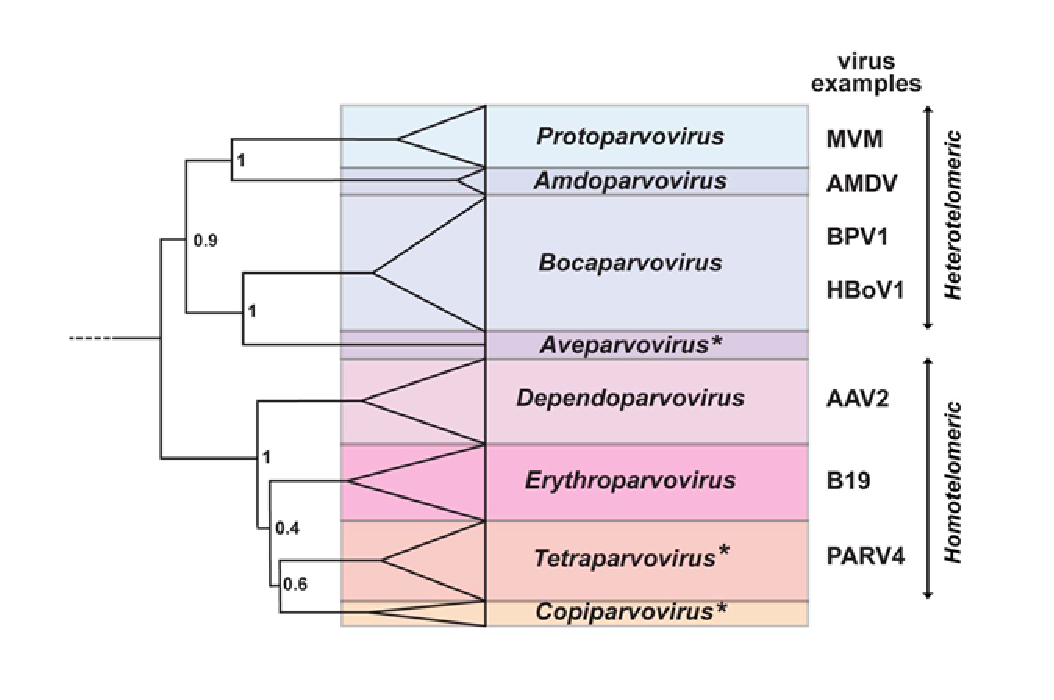
\includegraphics[width=\textwidth]{Taxonomy}
\caption[The \textit{Parvovirinae} subfamily]{The \textit{Parvovirinae} subfamily. The genera of the \textit{Parvovirinae} subfamily are depicted in a phylogenetic tree. Phylogenetic analysis is based on the amino acid sequence of the non-structural protein, NS1. The size of the color block for each genus indicates the relative number of species currently recognized, as an indicator of its diversity. Asterisks denote the names of new genera.} 
\label{Fig: Taxonomy}
\end{figure}



\section{The \textit{Parvovirinae} subfamily}
\label{sec: The Parvovirinae subfamily}   


\subsection{\textit{Amdoparvovirus}}

Mature virions exclusively contain negative strand genomic DNA of approximately 4.8 kb in length harbouring dissimilar palindromic sequences at each end \cite{pmid6252342, pmid2843669}. A single promoter located at map unit\footnotemark 3 at the left end of the genome generates all mRNA transcripts of AMDV. \footnotetext{Map units are commonly accepted units that relate to the position in the genome. The parvoviral genomes are arbitrarily subdivided into 100 map units (m.~u.).} Polyadenylation may occur at either the proximal site or at the distal site of the genome. Thus, the transcription profile of the genus \textit{Amdoparvovirus} most closely resembles  that of the genus \textit{Erythroparvovirus} \cite{pmid16378968}.  
Only two distant species have been reported. Firstly, \textit{Carnivore amdoparvovirus 1}, which comprises only Aleutian mink disease virus (AMDV) and secondly, \textit{Carnivore amdoparvovirus 2}, which encompasses solely gray fox amdovirus (GFAV) \cite{pmid22000359}. 
Permissive replication is tightly restricted to Crandell feline kidney cells. The virion surface displays three mounds elevated around the threefold icosahedral axis of symmetry. Several structure features were ascertained to be similar to those found in B19V, CPV, FPV, and MVM. Such appearance is comparable to those observed for the genus \textit{Dependoparvovirus} \cite{pmid10400786}. Remarkably, there is no evidence of a phospholipase 2A enzymatic core within the naturally truncated N-VP1 terminus of members belonging to the genus \textit{Amdoparvovirus} as it is common to the other genera of the subfamily \textit{Parvovirinae} \cite{icvt}. 


\nomenclature{AMDV}{Aleutian mink disease virus}
\nomenclature{GFAV}{Gray fox amdovirus}
\nomenclature{PLA\textsubscript{2}}{Phospholipase A2}

\subsection{\textit{Aveparvovirus}}

\textit{Aveparvovirus} is a new genus within the \textit{Parvovirinae} subfamily that comprises of the species chicken parvovirus and turkey parvovirus. The name \textit{Aveparvovirus} is derived from \underline{av}ian parvoviruses, referring to the hosts from which the members were isolated. Although these viruses were identified for years in the intestinal tracts of poultry \cite{pmid18766849, pmid6847550, pmid2995561}, analysis of the complete nucleotide sequence has been reported only recently. Phylogenetic study of the genomic sequences revealed that interestingly, ChPV and TuPV do not group phylogenetically with GPV and DPV, that are members of the genus \textit{Dependoparvovirus}. It was clearly demonstrated that ChPV, along with the closely related TuPV, represents the prototype of a novel genus within the \textit{Parvovirinae} subfamily \cite{pmid25510852, pmid18622862}. Identical direct repeat sequences flank the genome at both the 3' and the 5' end. Each of which contains a 39 nt ITR that is predicted to form a hairpin structure. ChPV and TuPV feature an overall genome organization similar to that of members of the genus \textit{Bocaparvovirus} \cite{pmid20097398}. 
Although it has been demonstrated that ChPV can induce clinical signs in broiler chickens that show characteristics of the runting-stunting syndrome (RSS) \cite{pmid18766892}, the role of avian parvoviruses in the aetiology of enteric diseases in poultry still remains to be demonstrated. RSS, also referred to as malabsorption syndrome, is characterized by significantly decreased egg hatchability, poorly developed hatched chickens, serious growth retardation, diarrhoea, enteritis, disturbed feathering, low vitality, and bone disorders \cite{pmid7150147, pmid6281962, pmid8363509}. Currently, the pathogenicity of TuPV has not been investigated yet. The predominant enteric diseases in turkeys are known as poult enteritis complex (PEC) \cite{pmid10935280} or the more drastic poult enteritis mortality syndrome (PEMS) \cite{PEMS}. Understanding the role of avian parvoviruses in PEMS, PEC, and RSS is of great interest due to the economic losses resulting from enteric diseases in poultry. \cite{pmid18622862}. 
  
    



\nomenclature{ChPV}{Chicken parvovirus}
\nomenclature{TuPV}{Turkey parvovirus} 
\nomenclature{GPV}{Goose parvovirus}
\nomenclature{DPV}{Duck parvovirus}
\nomenclature{RSS}{Runting-stunting syndrome}
\nomenclature{PEC}{Poult enteritis complex}
\nomenclature{PEMS}{Poult enteritis mortality syndrome}


\subsection{\textit{Bocaparvovirus}}
The name of the genus is derived from \underline{bo}vine and \underline{ca}nine, referring to the two hosts of the first identified members of this genus.  The genomes of members of the genus \textit{Bocaparvovirus} are quite distinct from all other viruses in the subfamily \textit{Parvovirinae}. As the members of the genera \textit{Protoparvovirus} and \textit{Amdoparvovirus} they contain non-identical imperfect palindromic sequences at both ends of their 5.5 kb genome. Mature virions contain mainly, but not exclusively, negative strand ssDNA \cite{pmid3783814,pmid12441065}.
All RNA transcripts are generated from a single P4 promoter at the left-hand end of the genome. The transcripts are alternatively spliced and polyadenylated either at an internal site or at the 3’-end of the genome \cite{pmid17715221}. Noteworthy, bovine parvovirus (BPV), the main representative, encodes a 22.5 kDa nuclear phosphoprotein, NP1, whose function still remains unknown. This protein is distinct from any other parvovirus-encoded polypeptide \cite{pmid6319731}.
A human bocavirus was first described in 2005, when it was detected in nasopharyngeal aspirates of young children with respiratory tract infection \cite{pmid11562506, pmid16118271}. More recently, HBoV has been identified in diarrheal feces of children with gastroenteritis \cite{pmid17553287}. HBoV infection is associated with acute respiratory symptoms and is usually detected in children under 2 years of age \cite{pmid17122013, pmid16517912, pmid17041855}. HBoV infections have been reported world-wide and HBoV was often isolated in respiratory samples of diseased as well as asymptomatic patients sometimes long after the primary infection. Therefore, it can be frequently detected even though it is not likely acting as a pathogen, thus complicating the use of PCR in diagnostics. Furthermore, long-term persistence may explain that HBoV infection among adults was predominantly reported in association with immunosuppression or immunodeficiency \cite{pmid17041855, pmid17176591}.         



\nomenclature{BPV}{Bovine parvovirus}
\nomenclature{kDa}{Kilodalton}
\nomenclature{Da}{Dalton}


\subsection{\textit{Copiparvovirus}}
Based on phylogenetic analysis, the genus \textit{Copiparvovirus} encompasses PPV4 and BPV2. PPV4 was identified in clinical samples from swine herds \cite{pmid20339886, pmid21092136, pmid22967311} and represents a distinct branch together with BPV2 \cite{pmid11562506}. The name \textit{Copiparvovirus} refers to \underline{co}ws and \underline{pi}gs, the hosts from which members of that genus were isolated. PPV4 is unique in that it is phylogenetically most closely related to BPV2 but the coding capacity and genome organization resemble more those of viruses of the genus \textit{Bocaparvovirus}. While the ORF3 encoded proteins of the three recognized \textit{Bocaparvovirus} members share amino acid identities of 43.3-47.0~\% among themselves, the PPV4 ORF3 encoded protein does not display homology with any protein in the GenBank database \cite{pmid20339886, pmid21092136}. 
Recently, two novel porcine parvoviruses, PPV5 and PPV6, were discovered \cite{pmid23405295, pmid25442288}. Characterization of their nucleotide sequences revealed that their full-length genomes are approximately 6 kb in length. As a consequence of this capacious genome size, especially their capsid protein encoding genes are exceptionally large. Interestingly, the genomic organization of PPV5 and PPV6 is different from PPV4 in that they lack the extra ORF3 in the middle of the genome. Moreover, PPV5 as well as PPV6 possess the conserved putative secretory PLA\textsubscript{2} motif which is present in the capsid protein of most parvoviruses but is lacking in PPV4. In spite of considerable differences in the genomic organization between BPV2, PPV5, and PPV6 on the one hand and PPV4 on the other hand, phylogenetic analysis revealed a close evolutionary relationship of these viruses, suggesting that they share the same immediate ancestor \cite{pmid23762339, pmid25442288}.      
Since members of the genus \textit{Copiparvovirus} were discovered quite recently, their biological characteristics, relatedness to disease, and potential clinical manifestations are still not fully understood \cite{pmid20339886, pmid21092136, pmid23762339, pmid25442288}. Especially, Kresse strain of porcine parvovirus belonging to the genus \textit{Protoparvovirus} is known to be an important pathogen responsible for embryonic and fetal death in piglets, resulting in considerable losses in the pig industry worldwide \cite{pmid6314634, pmid427636, pmid999067, pmid3006323}. In order to clarify the precise role of the most recently discovered members of the genus \textit{Copiparvovirus} as causative agents of reproductive failure in breeding animals, more comprehensive epidemiologic studies are required in the future \cite{pmid25442288}. 



\subsection{\textit{Dependoparvovirus}}
Positive and negative strand ssDNA is distributed indifferently among mature virions belonging to the genus \textit{Dependoparvovirus} \cite{pmid5014934, pmid5264145}. The 4.7 kb DNA molecule contains identical ITRs of 145 nt, the first 125 nt of which form a palindromic sequence \cite{pmid6246271}. Three mRNA promoters that are located at map units 5, 19, and 40 initiate transcription that can be terminated in two polyadenylation sites located at the right-hand end or alternatively, in the middle of the genome \cite{pmid6253077, pmid6281463}. Common for all currently accepted replication-defective members of the genus \textit{Dependoparvovirus} is their strict dependence upon helper adenoviruses or herpesviruses \cite{pmid4318977, pmid6270377, pmid5227666}. Therefore, their host range tropism strongly depends on the one of the helper virus. 
The only exceptions are the autonomously replicating duck and goose parvoviruses which are also comprised within the \textit{Dependoparvovirus} genus based on phylogenetic analysis \cite{icvt}. The most important members of this genus are the adeno-associated viruses (AAV). They attracted considerable interests since at least one of them, AAV-2, has been reported to integrate site-specifically into human chromosome 19 \cite{pmid2156265, pmid1653762, pmid1334463, pmid1657596}. This characteristic makes AAV a promising candidate for creating viral vectors for gene therapy \cite{pmid18854481, pmid21499295}. As a well characterized member of the \textit{Dependoparvoviruses} AAV-2 represents the model virus among this genus.  


\subsection{\textit{Erythroparvovirus}}
Equivalent numbers of positive and negative sense ssDNA are packaged into infectious virions of the genus \textit{Erythroparvovirus}. As in the case with the genus \textit{Dependoparvovirus}, the 5.5 kb ssDNA molecule contains identical ITRs of 383 nt in length at both the 3’ and the 5’ end. The first 365 nt of those secondary elements form palindromic sequences \cite{pmid2408228}. Transcription is regulated by a single mRNA promoter located at map unit 6 \cite{pmid3824910}. A distal polyadenylation site for use in termination of RNA synthesis is located at the far right side. Additionally, transcripts may be terminated at an unusual internal polyadanylation site in the middle of the genome \cite{pmid3599180}. Viruses belonging to this genus are highly erythrotropic, meaning that efficient replication only occurs in rapidly dividing erythroid progenitor cells (EPCs) such as erythroblasts and megakaryocytes present in the bone marrow.
B19V, a widespread human pathogen that causes fifth disease, polyarthropathia, anemic crises in children with underlying hematological diseases (e.g. sickle cell anemia or thalassemia) and intrauterine infections (with hydrops fetalis in some cases) \cite{pmid12097253} represents the model virus among the genus \textit{Erythroparvovirus}. 

\nomenclature{Nt}{Nucleotide}
\nomenclature{ITR}{Inverted terminal repeat}
\nomenclature{Kb}{Kilo base}
\nomenclature{EPC}{Erythroid progenitor cell}


\subsection{\textit{Protoparvovirus}}
Kilham Rat virus (KRV), a member of the genus \textit{Protoparvoviruses} was the first member of the subfamily \textit{Parvovirinae} to be discovered in 1959 \cite{pmid13669314}. Some members of the genus contain positive strand DNA in variable proportions up to 50~\% \cite{pmid6694260}. However, in mature virions of most members, virtually only negative strand DNA occurs. What they have in common are their hairpin structures at both the 5’ and 3’ ends of the linear 5 kb ssDNA molecule that differ in both sequence and predicted structure \cite{pmid6298737}. Transcription of the genome is regulated by two mRNA promoters at map units 4 and 38 \cite{pmid6828378}. There is only one polyadenylation site at the 3’ end. 
Viral replication provokes characteristic cytopathic effects in cell culture. Many species display hemagglutination with erythrocytes of one or several species, but not enforcedly of their natural host \cite{pmid5083410}. The genus \textit{Protoparvovirus} is primarily represented by MVM \cite{icvt, protoparvovirus}.       

\nomenclature{KRV}{Kilham rat virus}

\subsection{\textit{Tetraparvovirus}}
The genus \textit{Tetraparvovirus} is a new genus that arose recently. To date, six species have been discovered, which were isolated from humans \cite{pmid15956568}, chimpanzees, baboons \cite{pmid20668071}, cows, pigs \cite{pmid18632954, pmid20653980, pmid22247522}, as well as sheep \cite{pmid21980506}. RNA transcripts that encode the NS-proteins or the VP-proteins are generated from two promoters that are located at map units 6 and 38, respectively. Transcription can be terminated in two polyadenylation sites located at the right-hand end of the genome or alternatively, at an internal polyadenylation site. Since the full-length genome has not been sequenced yet, information of the terminal repeats is still lacking \cite{pmid22044541}. Analysis of the NS1 protein revealed a G2/M cell cycle arrest induced in NS1-expressing hematopoietic stem cells that clearly involved the predicted helicase motifs \cite{pmid8106366, pmid9261429, pmid7966641} of NS1. To date, no PLA\textsubscript{2}-like activity of expressed VP1u polypeptides has been demonstrated for any member of the genus \textit{Tetraparvovirus} \cite{pmid22044541}. PARV4 is one of the only four groups of parvoviruses that is known to infect humans besides B19V, HBoV, and AAV. It was first reported in an intravenous drug user who was positive for HBV infection in 2005. The patient suffered from arthralgia, confusion, diarrhea, fatigue, neck stiffness, night sweat, pharyngitis, and vomiting. PARV4 represents a phylogenetic deeply rooted lineage between avian dependoviruses and bovine parvovirus type 3 \cite{pmid15956568}. So far, most evidence about PARV4 transmission comes from patients who had engaged in high risk behaviour for blood borne viral infections, where PARV4 infection basically was observed to be strongly associated with HCV and HIV infection \cite{pmid22492853, pmid22235298, pmid17397006}. However, there are several reports of parenteral transmission in the absence of HIV, HBC, or HCV. PARV4 IgG has been documented independently from other blood borne viruses among injecting drug users \cite{pmid23283958}, in haemophilia patients \cite{pmid22043925}, and in patients who were subjected to intra-muscular injections in the past \cite{pmid22469425}. Currently, no definitive clinical syndrome was associated with PARV4 infection and there is no evidence for a potential pathogenicity of related members of the genus \textit{Tetraparvovirus} in animals \cite{pmid18632954}. PARV4 viraemia appears to be asymptomatic \cite{pmid20587191} and co-existing blood borne viruses do not increase severity \cite{pmid22235298}.   

  








 


\nomenclature{PARV4}{Parvovirus 4}
\nomenclature{HBoV}{Human Bocavirus}
\nomenclature{HIV}{Human immunodeficiency virus}
\nomenclature{HCV}{Hepatitis C virus}
\nomenclature{HBV}{Hepatitis B virus}
\nomenclature{ORF}{Open reading frame}
\nomenclature{VP1u}{VP1 unique region}

\clearpage



\begin{tiny}
\begin{center}

\begin{longtable}{p{0.7in} p{1.65in} p{1.6in} p{0.6in} p{0.65in}}
\caption[Taxonomy for the subfamily \textit{Parvovirinae}]{Taxonomy for the subfamily \textit{Parvovirinae}}\\
\\
\label{Tab: Taxonomy}
\textbf{Genus} & \textbf{Species} & \textbf{Virus or virus variants} & \textbf{Abbr.} & \textbf{ACNO}\footnotemark\\
\hline
\endfirsthead % all the lines above this will be repeated on every page

\multicolumn{3}{l}{\normalsize\textbf{Table~\ref{Tab: Taxonomy}} continued}\\
\\
\textbf{Genus} & \textbf{Species} & \textbf{Virus or virus variants} & \textbf{Abbr.} & \textbf{ACNO}\\
\hline
\endhead

\hline
\multicolumn{5}{l}{The type species for each genus is indicated in bold type. \cite{pmid24212889}}
\endlastfoot

\textit{Amdoparvovirus} & \textbf{\textit{Carnivore amdoparvovirus 1}} & Aleutian mink disease virus & AMDV & JN040434 \\
 & \textit{Carnivore amdoparvovirus 2} & Gray fox amdovirus & GFAV & JN202450 \\
\textit{Aveparvovirus} & \textit{\textbf{Galliform aveparvovirus 1}} & Chicken parvovirus & ChPV & GU214704 \\
& & Turkey parvovirus & TuPV & GU214706 \\
\textit{Bocaparvovirus} & \textit{Carnivore bocaparvovirus 1} & Canine minute virus & CnMV & FJ214110 \\
& \textit{Carnivore bocaparvovirus 2} & Canine bocavirus 1 & CBoV & JN648103 \\
& \textit{Carnivore bocaparvovirus 3} & Feline bocavirus & FBoV & JQ692585 \\
& \textit{Pinniped bocaparvovirus 1} & California sea lion bocavirus 1 & CslBoV1 & JN420361\\
& & California sea lion bocavirus 2 & CslBoV2 & JN420366 \\
& \textit{Pinniped bocaparvovirus 2} & California sea lion bocavirus 3 & CslBoV3 & JN420365 \\
 & \textit{Primate bocaparvovirus 1} & Human bocavirus 1 & HBoV1 & JQ923422 \\
 & & Human bocavirus 3 & HBoV3 & EU918736 \\
 & & Gorilla bocavirus & GBoV & HM145750 \\
 & \textit{Primate bocaparvovirus 2} & Human bocavirus 2a & HBoV2a & FJ973558 \\
 & & Human bocavirus 2b & HBoV2b & FJ973560 \\
 & & Human bocavirus 2c & HBoV2c & FJ170278 \\
 & & Human bocavirus 4 & HBoV4 & FJ973561 \\
 & \textit{\textbf{Ungulate bocaparvovirus 1}} & Bovine parvovirus & BPV & DQ335247 \\
 & \textit{Ungulate bocaparvovirus 2} & Porcine bocavirus 1 & PBoV1 & HM053693 \\ 
 & & Porcine bocavirus 2 & PBoV2 & HM053694 \\
 & & Porcine bocavirus 6 & PBoV6 & HQ291309 \\
 & \textit{Ungulate bocaparvovirus 3} & Porcine bocavirus 5 & PBoV5 & HQ223038 \\
 & \textit{Ungulate bocaparvovirus 4} & Porcine bocavirus 7 & PBoV7 & HQ291308 \\ 
 & \textit{Ungulate bocaparvovirus 5} & Porcine bocavirus 3 & PBoV3 & JF429834 \\ 
 & & Porcine bocavirus 4-1 & PBoV4-1 & JF429835 \\
 & & Porcine bocavirus 4-2 & PBoV4-2 & JF429836 \\
 \textit{Copiparvovirus} & \textit{\textbf{Ungulate copiparvovirus 1}} & Bovine parvovirus 2 & BPV2 & AF406966 \\
 & \textit{Ungulate copiparvovirus 2} & Porcine parvovirus 4 & PPV4 & GQ387499 \\
 \textit{Dependoparvovirus} & \textit{\textbf{Adeno-associated dependoparvovirus A}} & Adeno-associated virus-1 & AAV1 & AF063497 \\ 
 & & Adeno-associated virus-2 & AAV2 & AF043303 \\
 & & Adeno-associated virus-3 & AAV3 & AF028705 \\
 & & Adeno-associated virus-4 & AAV4 & U89790 \\
 & & Adeno-associated virus-6 & AAV6 & AF028704 \\
 & & Adeno-associated virus-7 & AAV7 & AF513851 \\
 & & Adeno-associated virus-8 & AAV8 & AF513852 \\
 & & Adeno-associated virus-9 & AAV9 & AX753250 \\
 & & Adeno-associated virus-10 & AAV10 & AY631965 \\ 
 & & Adeno-associated virus-11 & AAV11 & AY631966 \\ 
 & & Adeno-associated virus-12 & AAV12 & DQ813647 \\
 & & Adeno-associated virus-13 & AAV13 & EU285562 \\
 & & Adeno-associated virus-S17 & AAVS17 & AY695376 \\
 & \textit{Adeno-associated dependovirus B} & Adeno-associated virus-5 & AAV5 & AF085716 \\
 & & Bovine adeno-associated virus & BAAV & AY388617 \\
 & & Caprine adeno-associated virus & CapAAV & DQ335246 \\
 & \textit{Anseriform dependoparvovirus 1} & Duck parvovirus & DPV & U22967 \\
 & & Goose parvovirus-PT & GPV2 & JF926695 \\
 & & Goose parvovirus & GPV & U25749 \\
 & \textit{Avian dependovirus 1} & Avian adeno-associated virus & AAAV & AY186198 \\
 & \textit{Chiropteran dependoparvovirus 1} & Bat adeno-associated virus & BtAAV & GU226971 \\
 & \textit{Pinniped dependoparvovirus 1} & California sea lion adeno-associated virus & CslAAV & JN420372 \\
 & \textit{Squamate dependoparvovirus 1} & Snake adeno-associated virus & SAAV & AY349010 \\
 \textit{Erythroparvovirus} & \textit{\textbf{Primate erythroparvovirus 1}} & Human parvovirus B19-Au & B19V-Au & M13178 \\
 & & Human parvovirus B19-J35 & B19V-J35 & AY386330 \\
 & & Human parvovirus B19-Wi & B19V-Wi & M24682 \\
 & & Human parvovirus B19-A6 & B19V-A6 & AY064475 \\
 & & Human parvovirus B19-Lali & B19V-Lali & AY044266 \\
 & & Human parvovirus B19-V9 & B19V-V9 & AJ249437 \\
 & & Human parvovirus B19-D91 & B19V-D91 & AY083234 \\
 & \textit{Primate erythroparvovirus 2} & Simian parvovirus & SPV & U26342 \\
 & \textit{Primate erythroparvovirus 3} & Rhesus macaque parvovirus & RhMPV & AF221122 \\
 & \textit{Primate erythroparvovirus 4} & Pig-tailed macaque parvovirus & PtMPV & AF221123 \\
 & \textit{Rodent erythroparvovirus 1} & Chipmunk parvovirus & ChpPV & GQ200736 \\
 & \textit{Ungulate erythroparvovirus 1} & Bovine parvovirus 3 & BPV3 & AF406967 \\
 \textit{Protoparvovirus} & \textit{Carnivore protoparvovirus 1} & Feline parvovirus & FPV & EU659111 \\ 
 & & Canine parvovirus & CPV & M19296 \\
 & & Mink enteritis virus & MEV & D00765 \\
 & & Racoon parvovirus & RaPV & JN867610 \\
 & \textit{Primate protoparvovirus 1} & Bufavirus 1a & BuPV1a & JX027296 \\
 & & Bufavirus 1b & BuPV1b & JX027295 \\
 & & Bufavirus 2 & BuPV2 & JX027297 \\
 & \textit{\textbf{Rodent protoparvovirus 1}} & H-1 parvovirus & H1 & X01457 \\
 & & Kilham rat virus & KRV & AF321230 \\
 & & LuIII virus & LuIII & M81888 \\
 & & Minute virus of mice (prototype) & MVMp & J02275 \\
 & & Minute virus of mice (immunosuppressive) & MVMi & M12032 \\
 & & Minute virus of mice (Missouri) & MVMm & DQ196317 \\
 & & Minute virus of mice (Cutter) & MVMc & U34256 \\
 & & Mouse parvovirus 1 & MPV1 & U12469 \\
 & & Mouse parvovirus 2 & MPV2 & DQ196319 \\
 & & Mouse parvovirus 3 & MPV3 & DQ199631 \\
 & & Mouse parvovirus 4 & MPV4 & FJ440683 \\
 & & Mouse parvovirus 5 & MPV5 & FJ441297 \\
 & & Hamster parvovirus & HaPV & U34255 \\ 
 & & Tumor virus X & TVX & In preparation \\
 & & Rat minute virus 1 & RMV1 & AF332882 \\
 & \textit{Rodent protoparvovirus 2} & Rat parvovirus 1 & RPV1 & AF036710 \\
 & \textit{Ungulate protoparvovirus 1} & Porcine parvovirus Kresse & PPV-Kr & U44978 \\
 & & Porcine parvovirus NADL-2 & PPV-NADL2 & L23427 \\
 \textit{Tetraparvovirus} & \textit{Chiropteran tetraparvovirus 1} & Eidolon Helvum (bat) parvovirus & Ba-PARV4 & JQ037753 \\
 & \textit{\textbf{Primate tetraparvovirus 1}} & Human parvovirus 4 G1 & PARV4G1 & AY622943 \\
 & & Human parv4 G2 & PARV4G2 & DQ873391 \\      
 & & Human parv4 G3 & PARV4G3 & EU874248 \\
 & & Chipmanzee parv4 & Ch-PARV4 & HQ113143 \\
 & \textit{Ungulate tetraparvovirus 1} & Bovine hokovirus 1 & B-PARV4-1 & EU200669 \\
 & & Bovine hokovirus 2 & B-PARV4-2 & JF504697 \\
 & \textit{Ungulate tetraparvovirus 2} & Porcine hokovirus & P-PARV4 & EU200677 \\
 & \textit{Ungulate tetraparvovirus 3} & Porcine Cn virus & CnP-PARV4 & GU938300 \\
 & \textit{Ungulate tetraparvovirus 4} & Ovine hokovirus & O-PARV4 & JF504699 \\
 



\label{Taxonomy for the subfamily Parvovirinae}
     
\end{longtable}
\end{center} 
\end{tiny}


\footnotetext{NIH GenBank accession number}
\nomenclature{NIH}{National institutes of health}

\newpage
